\xchapter{Metodologia}{}

%O processo de mineração de opinião
%\begin{itemize}

%\item Preprocessing
%\begin{itemize}
%\item Definição
%\item Reiterar o tipo de análise escolhida: Document Level Analysis
%\item Datasets utilizados (Cornell e Amazon - descreve as caracteristicas de cada dataset, como quantidade, balanceamento, natureza, etc.)
%
%\item Descrever e justificar as tarefas envolvidas:
%\begin{itemize}
%\item O texto é dividido em sentenças
%\item POS Tagging - Brill's Tagger
%\item Blocos irrealis são filtrados ou não (atualmente NÃO FILTRAM)
%\item Defino quais ngrams serão extraídos
%\begin{itemize}
%\item Defino o uso do tipo de negação (FAR NEGATION - REFER)
%\item Os verbos foram recentemente removidos do universo
%\item Depois de testar, MANUALMENTE, diferentes configurações de n-grams, mantendo os demais parametros fixos, restaram adjetivos e adverbios, com unigrams, bigrams e trigrams
%\end{itemize}
%
%\item Retorna um vetor de n-grams (bag-of-words)
%\item Resume o subcapitulo e finaliza falando da saída dessa fase para a próxima
%\end{itemize}
%\end{itemize}
%\end{itemize}

O processo de mineração de opinião é comumente definido em seis etapas: a i) definição do domínio, ii) pré-processamento, iii) transformação, iv) seleção de características, v) classificação e vi) análise dos resultados \cite{moraes2012document}. Cada etapa inclui diferentes tarefas que, dado um documento na entrada do processo, seja possível classifica-lo e avaliar a classificação realizada.

\begin{figure}[h]
\caption{Etapas do processo de mineração de opinião.}
\centering
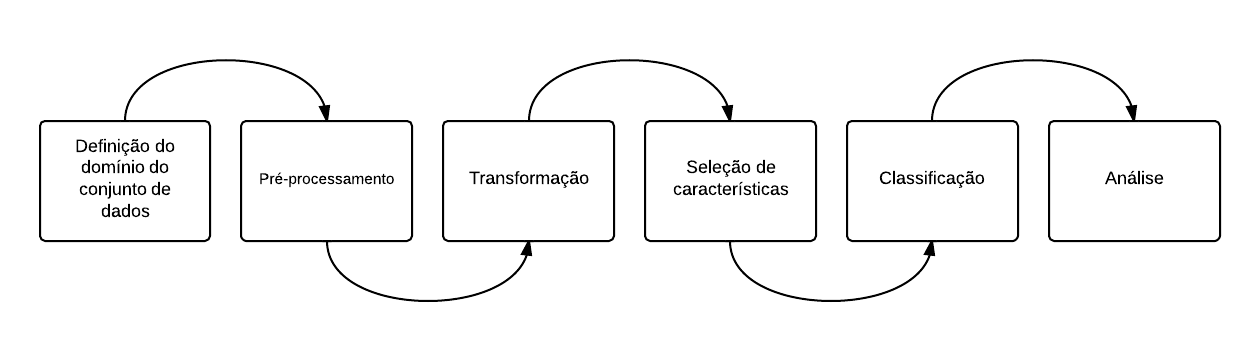
\includegraphics[scale=0.35]{opinion_mining_process.png}
\label{figura:processo_mineracao}
\end{figure}

\section{Definição do domínio e o pré-processamento dos dados}

Domínios diversos foram escolhidos para serem analisados por essa pesquisa, dentre eles filmes, livros, carros, computadores, panelas, hotéis, músicas, celulares, mp3, pen-drives, dispositivos gps, wifi e câmeras fotográficas. Essa diversidade de domínios é importante para que nós possamos corroborar nossa proposta de criar um classificador independente de domínio. Todas as bases de dados são da língua inglesa, pois os trabalhos relacionados a esta pesquisa utilizaram domínios nessa língua.

Para filmes, nós utilizamos a largamente utilizada \footnote{Vide https://www.cs.cornell.edu/people/pabo/movie-review-data/otherexperiments.html} base de dados, versão 2.0, desenvolvida e pré-classificada por \cite{pang2004sentimental}, com 2000 críticas de filmes, sendo metade positivas e outra metade negativas - bases assim, são conhecidas como balanceadas. As opiniões dos domínios de livros, carros, computadores, panelas, hotéis, músicas, celulares estão reunidos numa base de dados balanceada produzida por \cite{taboada2011lexicon}, retiradas do site Epinions \footnote{Vide http://www.epinions.com/}, com cerca de 400 críticas. E para as opiniões dos domínios de mp3, pen-drives, dispositivos gps, wifi e câmeras fotográficas, nós utilizamos uma base de dados balanceada de 2000 críticas retiradas do site da Amazon. 

Após a definição de um ou mais domínios é preciso, antes de inciar a etapa de pré-processamento, definir o nível da análise que será feita sobre os documentos. Existem três níveis básicos de análise de documentos em mineração de opinião: i) nível de análise de documento, ii) sentenças e iii) entidades e seus aspectos. O primeiro nível foca em classificar a opinião geral de um documento expressando-a como positiva ou negativa. O segundo nível, o de sentenças, em vez de considerar o sentimento geral das opiniões presentes em um documento como todo, classifica as opiniões de cada sentença separadamente. E o último nível foca em descobrir todos os alvos existentes nas sentenças do documento, e classifica as opiniões direcionadas a eles \cite{bing:2012}. Este trabalho decidiu utilizar o nível de análise de documento \cite{joachims1998text, pang2002thumbs, gamon2004sentiment, mullen2004sentiment, pang2004sentimental, cui2006comparative}.

A etapa de pré-processamento envolve tarefas como a tokenização dos documentos, marcação gramatical das palavras (do inglês, \textit{Part of Speech Tagging} ou POST), filtragem de sentenças com modais e definição os n-grams que serão utilizados para construir um modelo que represente o documento. A tokenização dos documentos é a tarefa que divide o conteúdo de cada documento em sentenças e, por sua vez, em palavras para que o marcador gramatical (ou \textit{tagger}) possa identificar as classes gramaticais das palavras do documento. O marcador gramatical usado foi o discutido em \cite{brill1995transformation} e usado em trabalhos relacionados a esta pesquisa \cite{chaovalit2005movie, taboada2008extracting, taboada2011lexicon}. A tarefa seguinte é a remoção de sentenças que possuem verbos modais. Segundo \cite{taboada2011lexicon}, modais como "would", "could", dentre outros, presentes numa sentença indicam que as palavras que aparecem juntamente com eles podem não ser confiáveis para serem usadas na definição do sentimento geral de opiniões de um documento. 

A tarefa final é definir quais n-grams serão usados para compor o modelo que representará o documento. O tipo de modelo utilizado nessa pesquisa é o popular saco de palavras (\textit{bag-of-words}), onde cada documento é representado por um vetor de termos (ou n-grams) do documento \cite{moraes2012document}. N-grams são termos que podem ser unigrams (uma palavra), bigrams (duas palavras) ou trigrams (três palavras). Nós definimos 5 tipos de n-grams: adjetivos e advérbios como unigrams; advérbios com adjetivos (e.g. \textit{very good}), advérbios com advérbios como bigrams; e a combinação de dois advérbios e um adjetivo como trigram (e.g. \textit{not very nice}) \cite{pang2002thumbs, turney2002thumbs, taboada2008extracting, karamibekr2012verb}. Nós também extraímos tipos especiais de bigrams e trigrams que são os n-grams negados (e.g. \textit{not bad}, \textit{nothing special}). A extração desses tipos de n-grams também é conhecido com detecção de negação e, por si só, é um linha de pesquisa completa, indo além do escopo deste trabalho. Nós utilizamos uma versão simplificada da técnica usada em \cite{taboada2011lexicon}. 

Ao fim do estágio de pré-processamento, cada documento é transformado num vetor de n-grams que é passado para a etapa de transformação. 

\section{Transformação}

%\item Transformation
%\begin{itemize}
%\item O que é
%\item Uso de dicionários de opinião para transformar n-grams e numeros
%\item Explicar porque o uso de dicionarios de opiniao é bom para nosso trabalho
%\item Sentiwordnet (falar sobre explicar, genericamente, como é criado, como é estruturado, valores associados aos termos)
%\item Falar do trabalho de Guerrine que propoe diferentes formulas para determinar a polaridade de um n-gram. E que são melhores que a mais frequente do SWN
%\item Falar e explicar os intensificadores
%\item Negação
%\item Frequencia de n-grams como transformador da polaridade
%\item Compensação de bias negativo
%\item Resume o subcapitulo e finaliza falando da saida dessa fase para a proxima 
%\end{itemize}

A etapa de transformação cria representações numéricas para os vetores de n-grams da etapa de pré-processamento, onde cada n-gram é associado a um valor numérico, um grau de polaridade opinativo, usando um dicionário de opiniões \cite{ballhysa2012fuzzy, moraes2012document, mouthami2013sentiment}. O dicionário base de opiniões usado nesse trabalho foi o SentiWordNet 3.0 \footnote{Disponível em: http://sentiwordnet.isti.cnr.it/. Download de 22/01/2013} \cite{baccianella2010sentiwordnet}.

\subsection{SentiWordNet 3.0}

O SentiWordNet 3.0 (SWN) é a terceira versão d SentiWordNet 1.0, apresentada por \cite{esuli2006sentiwordnet}. É um dicionário criado pela anotação automática de todos os conjuntos de sinônimos cognitivos, chamados de \textit{synsets}, de outro dicionário, o WordNet, versão 3.0 \cite{fellbaum2005wordnet}. Esses synsets são anotados de acordo sua positividade, negatividade e neutralidade. Cada \textit{synset} $s$ é associado a três valores numéricos $Pos(s)$, $Neg(s)$ e $Obj(s)$ que indicam o quanto positivos, negativos e "objetivos" (ou neutros) são os termos existentes no \textit{synset} \cite{baccianella2010sentiwordnet}.
Por exemplo, o synset [estimable (J, 3)] \footnote{Nós adotamos a convenção usada no WordNet e por \cite{esuli2006sentiwordnet} e \cite{baccianella2010sentiwordnet} que usa o termo entre colchetes para representar um synset; assim [poor (J, 7)] não só se refere ao termo "poor", mas ao synset formado pelos adjetivos {inadequate(J,2), poor(J,7), short(J,4)}}, correspondente ao sentido de “may be computed or estimated” do adjetivo "estimable", tem o grau de neutralidade $Obj(s)$ de 1.0 (e de positividade $Pos(s)$ e negatividade $Neg(s)$ igual a zero), enquanto que o synset [estimable (J, 1)], correspondente ao sentido de “deserving of respect or high regard”, tem o grau de positividade $Pos(s)$ de 0.75, $Neg(s)$ de 0.0 e $Obj(s)$ de 0.25. Cada um dos valores estão num intervalo $[0, 1]$ e a soma dos três é igual a 1. Assim, é possível que existam (e existem) \textit{synsets} que tenham todos os três graus diferentes de zero, indicando que há termos positivos, negativos e objetivos ao mesmo tempo \cite{esuli2006sentiwordnet}.

Inicialmente, nós definimos a polaridade resultante $Pol(n)$ de um termo (ou unigram) $n$, marcado gramaticalmente (e.g. adjetivo, advérbio, etc.), como $Pol(n) = Pos(s) - Neg(s)$ ,subtraindo o grau de positividade do grau de negatividade do synset $s$ mais frequente a que pertence o unigram. Por exemplo, o synset mais freqüente de [good (J,1)] somente possui o termo \textit{good}, com grau $Pos(s)$ de 0.75, $Neg(s)$ de 0.0 e $Obj(s)$ de 0.25. A polaridade resultante $Pol(n)$ será de 0.5. Contudo, essa abordagem, de utilizar o synset mais frequente, não é melhor que escolher, aleatoriamente, um dos synsets. Além disso, o uso de polaridades de palavras fora de contexto (do inglês \textit{word’s prior polarity}), típicas de abordagens \textit{bag-of-words}, deve ter um tratamento diferente para se adequar ao problema da perda do contexto causada na etapa de pré-processamento, com a tokenização do documento  \cite{guerini2013sentiment}. Assim, nós utilizamos um dicionário derivado do SWN produzido por  \cite{guerini2013sentiment} com todas as polaridades fora de contexto calculadas de todos os termos do SentiWordNet 3.0. A polaridade resultante $Pol(n)$ agora é a polaridade fora de contexto do unigram. 

O uso da abordagem de polaridades fora de contexto tem a vantagem de não depender de profunda análise semântica ou desambiguação (uma linha de pesquisa completa, por si só) para assinalar um valor opinativo para um termo, além de ser independente de domínio, como proposto nesse trabalho \cite{guerini2013sentiment}. Além disso, dicionários construídos automaticamente, como o SWN e a variação de Guerrine, superam problemas existentes de dicionários criados manualmente, como em \cite{taboada2008extracting, taboada2011lexicon} que tendem a se restringir a um número muito menor de termos, consomem tempo para serem construídos e podem sofrer enviesamento de seus autores \cite{ohana2009sentiment}. Outra vantagem de usar técnicas baseadas em dicionários é que dispensa o uso de grandes bases de dados para aprendizado ou motores de buscas com funcionalidades especiais para a tarefa \cite{khan2011sentiment}. A principal desvantagem, todavia, é que a fase de  transformação depende inteiramente da cobertura do dicionário utilizado \cite{khan2011sentiment}. 

\subsection{Definição da polaridade}

\subsubsection{Unigrams}

Dado um unigram do vetor de n-grams de um documento, a polaridade deste é definida pela polaridade fora de contexto provida pelo dicionário de opiniões. Caso o unigram não seja encontrado no dicionário, o lema deste é utilizado. Se ainda assim, o dicionário não cobrir o unigram em questão, ele é descartado do processo.
Nós também analisamos a ocorrência do unigram no documento. A enésima ocorrência $n$ de um unigram no documento terá somente $1/n$ da polaridade original retirada do dicionário de opiniões. Por exemplo:

\textit{Overall, the movie was great. The acting was great, the history was great, and the direction was just plain great.}

A repetição da palavra \textit{great} sugere que a pessoa que escreveu a crítica acima não tinha um termo específico que expressasse outras opiniões e utilizou \textit{great} de maneira genérica. Outra razão para suavizar a polaridade de unigrams que se repetem é que uma palavra que aparece regularmente tem a mais probabilidade de ser um termo neutro \cite{taboada2011lexicon}. 

Outra análise relacionada a definição da polaridade de um unigram, foi o enviesamento positivo. Classificadores que utilizam dicionários de opiniões geralmente mostram uma tendência para classificar o sentimento geral de um documento para a positividade, devido a tendência natural do ser humano de utilizar linguagem positiva e evitar termos negativos \cite{boucher1969pollyanna, kennedy2006sentiment}. Para tentar dirimir esse enviesamento, nós utilizamos uma abordagem proposta por \cite{taboada2011lexicon} que consiste em aumentar em 50\% a polaridade de todo unigram negativo. 

\subsubsection{Bigrams e trigrams}

O dicionário de opiniões provê a polaridade somente para unigrams. Para os outros tipos de n-grams, bigrams e trigrams, tivemos de considerar a influência entre as palavras dos n-grams. Os bigrams e trigrams propostos nesse trabalho são compostos por advérbios e adjetivos ou somente por advérbios, conforme definimos na etapa de pré-processamento. Os advérbios que antecedem os adjetivos ou advérbios nos n-grams são chamados de modificadores, intensificadores ou atenuadores, pois eles alteram a polaridade das palavras que os acompanham \cite{voll2007not}. Os intensificadores aumentam o grau da polaridade do unigram, seja ele positivo ou negativo, e os atenuadores diminuem. Por exemplo, 

\begin{itemize}
\item \label{itm:very_exem} $Pos(\textit{good}) = 0,72259$; $Pos(\textit{very good}) = 0,90323$
\item \label{itm:really_exem} $Neg(\textit{bad}) = -0.44006$; $Neg(\textit{really bad}) = -0,5060$
\end{itemize}

Os advérbios \textit{very} e \textit{really} modificam as polaridades dos adjetivos de \textit{good} e \textit{bad}. Diferentemente de dicionários de opiniões, como o SWN e a variação de Guerrine, não conseguimos encontrar, até o presente momento da pesquisa, nenhuma fonte disponível de intensificadores e amenizadores. Diferentes autores como \cite{voll2007not}, \cite{taboada2008extracting}, \cite{taboada2011lexicon} e \cite{pimpalkar2013sentimental} citam alguns modificadores ou até mencionam que construíram, manualmente, dicionários de modificadores próprios, mas não disponibilizaram tais recursos para serem reproduzidos nessa pesquisa. Assim, tivemos de construir nosso próprio dicionário de modificadores. 

Do mesmo modo que não há dicionários de intensificadores e amenizadores disponíveis nessa área de pesquisa, também não há consenso de como a modificação dos adjetivos pelos advérbios é feita. Nós decidimos nos basear no trabalho de \cite{taboada2011lexicon} que acrescenta ou diminui um percentual da polaridade dos adjetivos, a depender das classes dos advérbios. \citeauthoronline{taboada2011lexicon} define uma lista inicial (\ref{table:adv_seed}) de advérbios para criar seu dicionário e nós usamos a mesma lista para criar o nosso.

\begin{table}[!h]
	\centering
    \begin{tabular}{lll}
    Advérbio         				& Classe          & Percentual modificador \\ \hline
    pretty                   			& LOW 			   & -10\% \\
    somewhat                   	& VERY LOW  & -30\% \\
    slightly                   		& LOWEST 	   & -50\% \\
    really                   			& HIGH 			   & 15\% \\
    very                   			& VERY HIGH &  25\% \\
    extraordinarily             & HIGHEST 	   & 50\% \\
    most                   			& MOST HIGHEST & 100\% \\
    \end{tabular}
    \caption{Lista inicial de advérbios retirada de \cite{taboada2011lexicon}}
	\label{table:adv_seed}
\end{table}

Diferentemente do que foi feito em \citeauthoronline{taboada2011lexicon}, nós construímos o dicionário de modificadores automaticamente. Todos os advérbios existentes do Wordnet foram extraídos e, um a um, baseando-se na distância entre eles (os advérbios são organizados num grafo) e os advérbios da lista inicial, foram sendo associados aos advérbios iniciais. Por exemplo, o advérbio \textit{truly} é mais próximo de \textit{very}, da classe VERY HIGH, do que o advérbio \textit{really}, assim ele é associado à classe de \textit{very}. Um outro exemplo é \textit{fairly} que é mais próximo de \textit{somewhat} que do advérbio \textit{pretty}. A partir daí o cálculo polaridades dos bigrams pode ser calculados. Para as polaridades dos trigrams, o cálculo é análogo: primeiro calcula-se a polaridade do bigram mais interno e em seguida aplica-se o modificador mais externo a polaridade do bigram.

Existe ainda um tipo especial de n-gram que é a negação. São todos os n-grams formados por advérbios de negação e por adjetivos ou por advérbios. A abordagem inicial é inverter a polaridade do n-gram, mudando $Pos(\textit{good}) = 0,72259$ para $Pos(\textit{not good}) = - 0,72259$. Essa abordagem é conhecida como interruptor da negação ou inversão \cite{sauri2008factuality}. Contudo, embora a negação seja um efeito moderadamente local, é preciso analisar o efeito de palavras de negação, como \textit{none}, \textit{nobody} e \textit{nothing}, que tem efeito equivalente à negação local \cite{taboada2011lexicon} mas que atuam numa distância maior. Por exemplo:

\begin{example}
Nobody gives a good performance in this movie. (\textit{nobody} nega \textit{good})
\label{ex:far_neg_1}
\end{example}

\begin{example}
Out of every one of the fourteen tracks, none of them approach being weak and are all stellar. (\textit{none} nega \textit{weak})
\label{ex:far_neg_2}
\end{example}

Este trabalho utiliza uma versão simplificada da abordagem de \cite{das2001yahoo} para tentar englobar o efeito de maior distância da negação. Daí, ainda na etapa de pré-processamento, quando uma palavra de negação \footnote{As palavras de negação são: \textit{nobody}, \textit{none}, \textit{nothing}, \textit{not}, \textit{don't}, \textit{no}, \textit{doesn't}, \textit{isn't}, \textit{aren't}} era encontrada, todas as seguintes, até ser encontrado um ponto de fim de sentença, eram associadas ao advérbio \textit{not}, simbolizando a negação, criando, assim, bigrams ou trigrams. Se os n-grams criados se encaixassem na definição da etapa de pré-processamento, eram passados para essa etapa. 

A distância do efeito da negação também implica em como calcular a polaridade de um n-gram. Embora a inversão da polaridade funcione em certos casos como \textit{good} e \textit{not good} \cite{choi2008learning}, ele falha muito em outros \cite{liu2009review}. Considere o adjetivo \textit{awesome}, um adjetivo positivo $Pos(s) = 0.71506 $: se aplicarmos a inversão de polaridade, nós temos \textit{not awesome}, que é intuitivamente menos negativo que $Neg(\textit{terrible}) = -0.72503$. De fato, \textit{not awesome} parece ser mais positivo que \textit{not fine}, que aplicando a inversão, temos -0.37506. Para também englobar esse efeito da negação, nós usamos a abordagem proposta por \cite{taboada2011lexicon}, chamada de \textit{shift negation}. Em vez de inverter os sinais da polaridade, o grau de opinião do n-gram é deslocado em direção à polaridade oposta por um valor fixo (em nossa implementacão, 0.75). Por exemplo:

\begin{example}
She is not amazing (0,68 - 0,75 = -0,06) but not terrible (-0,72503 + 0,75 = 0,02497) either.
\label{ex:shift_1}
\end{example}

A negação de um termo fortemente positivo ou negativo reflete a mistura de opiniões que é corretamente capturada pelo deslocamento da negação \cite{taboada2011lexicon}. Ao fim da etapa de transformação, os vetores de n-grams são transformados em vetores numéricos de polaridades ou de graus de opiniões.  

\section{Seleção de características}

\section{Classificação}

\section{Avaliação}

\section{Design dos experimentos}